\usetikzlibrary {perspective} 

\newcommand\simplecuboid[7]{%
% drawing the contours
    % these ones connnect to the origin
    \fill[#7]  (xyz cs:x=#1+#4,y=#2,z=#3)
    -- (xyz cs:x=#1+#4,y=#2,z=#3+#6)
    -- (xyz cs:x=#1+#4,y=#2+#5,z=#3+#6)
    -- (xyz cs:x=#1+#4,y=#2+#5,z=#3) -- cycle;
    \fill[#7!50!white] (xyz cs:x=#1,y=#2+#5,z=#3)
    -- (xyz cs:x=#1,y=#2+#5,z=#3+#6)
    -- (xyz cs:x=#1+#4,y=#2+#5,z=#3+#6)
    -- (xyz cs:x=#1+#4,y=#2+#5,z=#3) -- cycle;
    \fill[#7!80!white] (xyz cs:x=#1,y=#2,z=#3)
    -- (xyz cs:x=#1,y=#2+#5,z=#3)
    -- (xyz cs:x=#1+#4,y=#2+#5,z=#3)
    -- (xyz cs:x=#1+#4,y=#2,z=#3) -- cycle;

    % \draw[black,thick] (xyz cs:x=#1,y=#2,z=#3) -- (xyz cs:x=#1,y=#2,z=#3+#6);
    % these are the 3 lines to be annotated with the number of channels and dimensions
    \draw[#7!50!black,thick] (xyz cs:x=#1,y=#2,z=#3) -- (xyz cs:x=#1,y=#2+#5,z=#3);
    \draw[#7!50!black,thick] (xyz cs:x=#1,y=#2,z=#3) -- (xyz cs:x=#1+#4,y=#2,z=#3);
    \draw[#7!50!black,thick] (xyz cs:x=#1+#4,y=#2,z=#3) -- (xyz cs:x=#1+#4,y=#2,z=#3+#6); % no of channels


    \draw[#7!50!black,thick] (xyz cs:x=#1+#4,y=#2,z=#3) -- (xyz cs:x=#1+#4,y=#2+#5,z=#3);
    \draw[#7!50!black,thick] (xyz cs:x=#1,y=#2+#5,z=#3+#6) -- (xyz cs:x=#1,y=#2+#5,z=#3);
    \draw[#7!50!black,thick] (xyz cs:x=#1,y=#2+#5,z=#3) -- (xyz cs:x=#1+#4,y=#2+#5,z=#3);
    \draw[#7!50!black,thick] (xyz cs:x=#1+#4,y=#2+#5,z=#3) -- (xyz cs:x=#1+#4,y=#2+#5,z=#3+#6);
    \draw[#7!50!black,thick] (xyz cs:x=#1+#4,y=#2+#5,z=#3+#6) -- (xyz cs:x=#1+#4,y=#2,z=#3+#6);
    \draw[#7!50!black,thick] (xyz cs:x=#1,y=#2+#5,z=#3+#6) -- (xyz cs:x=#1+#4,y=#2+#5,z=#3+#6);
    }

\newcommand\cnnblock[8]{
    
    % args 1 to 7 are the coordinates and colour of the simple cuboid
    % arg 8 says the annotation of the z coordinate
    \simplecuboid{#1}{#2}{#3}{#4}{#5}{#6}{#7}
    % annotated here in the cnn block
    
    \draw[#7!50!black,thick] (xyz cs:x=#1+#4,y=#2,z=#3) -- (xyz cs:x=#1+#4,y=#2,z=#3+#6) node[black,midway,below] {#8}; % no of channels
}

\newcommand\annotatecnnx[6]{
    % arguments: x, y, z, deltaX, annotation, color
    \draw[#6!50!black,thick] (xyz cs:x=#1,y=#2,z=#3) -- (xyz cs:x=#1+#4,y=#2,z=#3) node[black,midway,below left] {#5};
}

\newcommand\annotatecnny[6]{
    % arguments: x, y, z, deltaY, annotation, color
    \draw[#6!50!black,thick] (xyz cs:x=#1,y=#2,z=#3) -- (xyz cs:x=#1,y=#2+#4,z=#3) node[black,midway,left] {#5};
}

\newcommand\fcblock[7]{
    % args: x,y,z, cuboidHeight, thickness, realHeight, color
    % \fcblock{-2.50}{-17.50}{358}{35}{5}{10}{red}
    \simplecuboid{#1}{#2}{#3}{#5}{#4}{#5}{#7}
    % annotate the number of inputs below the layer
    \draw[#7!50!black,thick] (xyz cs:x=#1+#5,y=#2,z=#3) -- (xyz cs:x=#1+#5,y=#2,z=#3+#5) node[black,midway,below] {#6}; % no of channels

}

\newcommand\transline[2]{
    \draw[black,thick] (xyz cs:x=0,y=0,z=#1) -- (xyz cs:x=0,y=0,z=#2);
}


% \newcommand\cubeface[4]{
%     \fill[fill=gray!#4,fill opacity=0.5] (tpp cs:x=(1,1),y=(0,#2),z=0)
%     -- (tpp cs:x=0,y=(1,#2),z=0)
%     -- (tpp cs:x=0,y=(1,#2),z=0)
%     -- (tpp cs:x=0,y=(0,#2),z=0) -- cycle;
% }

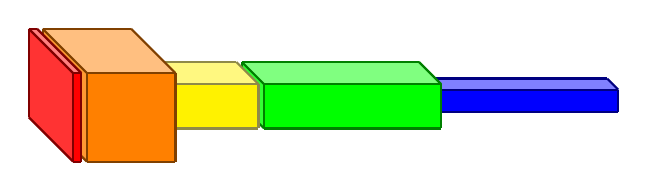
\begin{tikzpicture}[x={(0.5pt,-0.5pt)},y={(0pt,1pt)},z={(1pt,0pt)},thick]
    \simplecuboid{-4}{-4}{152}{8}{8}{64}{blue}{false}
    \simplecuboid{-8}{-8}{86}{16}{16}{64}{green}{false}
    \simplecuboid{-8}{-8}{52}{16}{16}{32}{yellow}{false}
    \simplecuboid{-16}{-16}{18}{32}{32}{32}{orange}{false}
    \simplecuboid{-16}{-16}{13}{32}{32}{3}{red}{true}
    \end{tikzpicture}

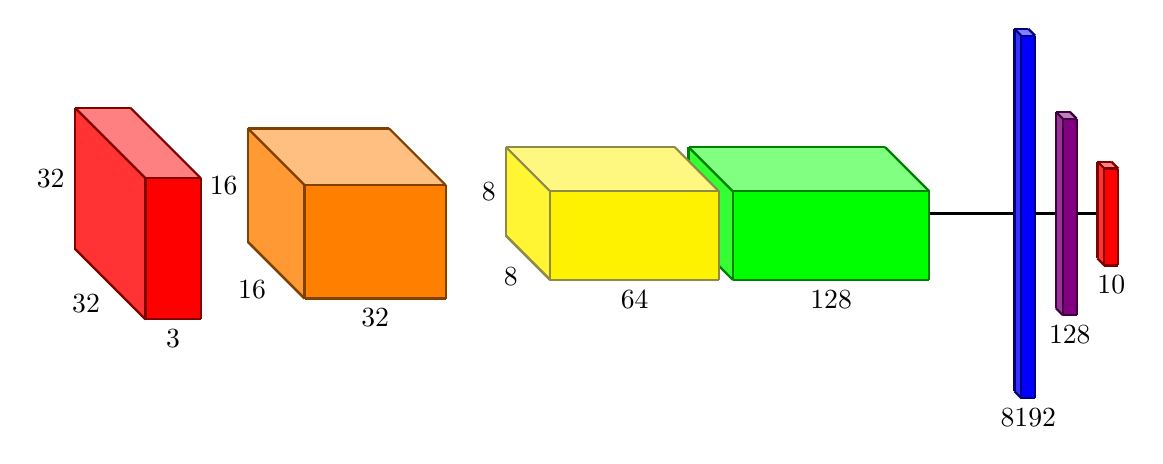
\begin{tikzpicture}[x={(0.5pt,-0.5pt)},y={(0pt,1pt)},z={(1pt,0pt)},thick]
\transline{343}{358}
\fcblock{-2.50}{-17.50}{358}{35}{5}{10}{red}
\transline{328}{343}
\fcblock{-2.50}{-35.50}{343}{71}{5}{128}{violet}
\transline{217}{328}
\fcblock{-2.50}{-65.50}{328}{131}{5}{8192}{blue}
\transline{151}{217}
\dashedconvol{-1}{-1}{288}{3}{3}{328}
\cnnblock{-16.00}{-16.00}{217}{32}{32}{71}{green}{128}
\dashedconvol{-1}{-1}{212}{3}{3}{217}
\cnnblock{-16.00}{-16.00}{151}{32}{32}{61}{yellow}{64}
\annotatecnnx{-16.00}{-16.00}{151.00}{32}{8}{yellow}
\annotatecnny{-16.00}{-16.00}{151.00}{32}{8}{yellow}
\dashedconvol{-1}{-1}{111}{3}{3}{151}
\cnnblock{-20.50}{-20.50}{60}{41}{41}{51}{orange}{32}
\annotatecnnx{-20.50}{-20.50}{60.00}{41}{16}{orange}
\annotatecnny{-20.50}{-20.50}{60.00}{41}{16}{orange}
\dashedconvol{-1}{-1}{20}{3}{3}{60}
\cnnblock{-25.50}{-25.50}{0}{51}{51}{20}{red}{3}
\annotatecnnx{-25.50}{-25.50}{0.00}{51}{32}{red}
\annotatecnny{-25.50}{-25.50}{0.00}{51}{32}{red}
\end{tikzpicture}



% \newcommand{\simpleaxes}[3]{%
%   \draw[->] (-0.5,0,0) -- (#1,0,0) node[pos=1.1]{x};
%   \draw[->] (0,-0.5,0) -- (0,#2,0) node[pos=1.1]{y};
%   \draw[->] (0,0,-0.5) -- (0,0,#3) node[pos=1.1]{z};}

% \begin{tikzpicture}[]
%     \draw plot coordinates{(1,0) (2,0.5) (3,0) (3,1)};
%     \draw[x={(0cm,1cm)},y={(1cm,0cm)},color=red]
%           plot coordinates{(1,0) (2,0.5) (3,0) (3,1)};
%   \end{tikzpicture}

% \begin{tikzpicture}[x={(0.5pt,-0.5pt)},y={(0pt,1pt)},z={(1pt,0pt)},thick]
%     \transline{200}{\textwidth}
%     \simplecuboid{0}{0}{0}{100}{100}{100}{blue}

%     \simplecuboid{-30}{-30}{20}{60}{60}{20}{orange}
%     \simplecuboid{-30}{-30}{10}{60}{60}{8}{green}
%     \transline{0}{10}
% \end{tikzpicture}

% \begin{tikzpicture}[x={(0.5pt,-0.5pt)},y={(0pt,1pt)},z={(1pt,0pt)},thick]
%     \simplecuboid{-4}{-4}{225}{8}{8}{64}{green}
%     \simplecuboid{-8}{-8}{156}{16}{16}{64}{green}
%     \simplecuboid{-8}{-8}{87}{16}{16}{32}{yellow}
%     \simplecuboid{-16}{-16}{50}{32}{32}{32}{yellow}
%     \simplecuboid{-16}{-16}{13}{32}{32}{3}{red}
%     \end{tikzpicture}

% This is another architecture


% \begin{tikzpicture}[x={(0.5pt,-0.5pt)},y={(0pt,1pt)},z={(1pt,0pt)},thick]
%     \simplecuboid{-4}{-4}{213}{8}{8}{64}{orange}
%     \simplecuboid{-8}{-8}{147}{16}{16}{64}{yellow}
%     \simplecuboid{-8}{-8}{81}{16}{16}{32}{green}
%     \simplecuboid{-16}{-16}{47}{32}{32}{32}{blue}
%     \simplecuboid{-16}{-16}{13}{32}{32}{3}{red}
%     \end{tikzpicture}

%     \begin{tikzpicture}[x={(0.5pt,-0.5pt)},y={(0pt,1pt)},z={(1pt,0pt)},thick]
%         \simplecuboid{-4}{-4}{152}{8}{8}{64}{blue}
%         \simplecuboid{-8}{-8}{86}{16}{16}{64}{green}
%         \simplecuboid{-8}{-8}{52}{16}{16}{32}{yellow}
%         \simplecuboid{-16}{-16}{18}{32}{32}{32}{orange}
%         \simplecuboid{-16}{-16}{13}{32}{32}{3}{red}
%         \end{tikzpicture}